
\fontsize{12}{12}\selectfont
\section{Image Blur}\label{sec:imageblur}
    \par A seguinte função visa a implementar um filtro de imagem de \textit{blur}, em que é aplicado um filtro da média de pixeis num dado retângulo de dimensão $(2dx + 1) \times (2dy + 1)$. \ Para tal, foram considerados dois algoritmos, detalhados nas subsecções seguintes.

\subsection{Algoritmo Melhorado}\label{subsec:blur1}
    \par Este algoritmo utiliza uma \href{https://en.wikipedia.org/wiki/Summed-area_table}{\textit{Summed-area table}}, definido por um \textit{array} bidimensional, com tamanho $width \times height$. \ Este pode ser dividido em duas partes: cálculo da soma das áreas em cada pixel e cálculo do \textit{blur} numa determinada área.

\subsubsection{Summed-area table}
    \par O seguinte método implementa uma forma de, em um dado ponto $(x,y)$, obter a soma de todos os valores dos pixeis desde $(0,0)$ a esse mesmo ponto. \ Da forma em que foi implementado, apenas é feita a média dos valores na atribuição na própria imagem, que resulta em o \textit{array} ser do tipo inteiro.

    \par A forma geral para a implementação deste algoritmo é:

    \begin{lstlisting}
      integral[x][y] = ImageGetPixel(img, x, y) +
      integral[x - 1][y] +
      integral[x][y - 1] -
      integral[x - 1][y - 1];    
    \end{lstlisting}

    \par Com o seguinte bloco de código, está a ser atribuído às coordenadas $(x,y)$ do \textit{array} criado anteriormente a soma total dos valores dos pixeis.
    \par Esta fórmula é visualmente representada na figura abaixo.

    \begin{figure} [H]
        \centering
        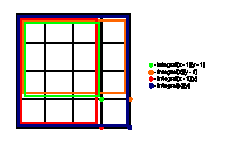
\includegraphics[scale=3]{images/sumareas.pdf}
        \caption{Figura ilustrativa do algoritmo \textit{Summed-area table}} 
    \end{figure}

    \newpage

    \par Ainda considerando o algoritmo anterior, Verifica-se um problema de \textit{assertion}, causado quando $x$ ou $y$ são 0. \ Para evitar esse problema, é atribuído inicialmente ao $(0,0)$ (já que a soma total nesse ponto é ele próprio) o seu próprio valor.

    \par De seguida, são preenchidas as linhas $x = 0$ e $y = 0$. \ Após isso, é possível preencher o resto do \textit{array} com a fórmula geral anteriormente apresentada.

\subsubsection{Média dos pixeis}
    \par O seguinte algoritmo é responsável por calcular a média dos pixeis numa determinada área, definida por um retângulo de dimensão $(2dx + 1) \times (2dy + 1)$. \ São usados os valores de soma obtidos na parte anterior.

    \par Inicialmente, são definidos o canto superior esquerdo e canto inferior direito, e verificar se o retângulo está dentro da imagem. \ Caso não esteja, é lhe atribuído o valor representante do extremo que está a ultrapassar.

    \par Finalmente, é calculada a média dos pixeis, com o seguinte bloco de código:

    \begin{lstlisting}
        (double)((integral[x2 - 1][y2 - 1] -
        integral[x1][y2 - 1] -
        integral[x2 - 1][y1] +
        integral[x1][y1])) /
        npixels + 0.5;
    \end{lstlisting}

    \par O valor de 0.5 é adicionado para que o valor seja arredondado corretamente, já que o valor é do tipo inteiro. \ Também é subtraído o valor de 1 a $x2$ e $y2$, de forma a que o valor seja o correto, já que o \textit{array} começa em $(0,0)$.

\subsubsection{Análise da Complexidade}
    \par Na seguite tabela, é possível observar a complexidade de cada função, em termos de iterações de ciclos e de operações aritméticas das duas partes do algoritmo.

    \begin{table}[H]
        \centering
        \begin{tabular}{| p{23mm} | p{25mm} | p{30mm} | p{30mm} | p{38mm} |}
            \hline

            \textbf{Imagem} & \textbf{Fator de \textit{blur}} & \textbf{Iterações de 3.1.1.} & \textbf{Iterações de 3.1.2} & \textbf{Complexidade} \\ \hline

            original.pgm (300x300) & $7,7$ & $90000$ & $90000$ & $O((width \times height) \times 2)$ \\ \hline

            original.pgm (300x300) & $40,40$ & $90000$ & $90000$ & $O((width \times height) \times 2)$ \\ \hline

            original.pgm (300x300) & $200,200$ & $90000$ & $90000$ & $O((width \times height) \times 2)$ \\ \hline

            airfield.pgm (1600x1200) & $40,40$ & $1920000$ & $1920000$ & $O((width \times height) \times 2)$ \\ \hline

            airfield.pgm (1600x1200) & $200,200$ & $1920000$ & $1920000$ & $O((width \times height) \times 2)$ \\ \hline

            ireland.pgm (640x480) & $40,40$ & $307200$ & $307200$ & $O((width \times height) \times 2)$ \\ \hline
        \end{tabular}
        \caption{Tabela com a complexidade das funções}
        \label{tab:complexidade}
    \end{table}

    \newpage

    \par Como é possível observar na tabela acima, a complexidade das funções é $O((width \times height) \times 2)$, já que o número de iterações é igual ao número de pixeis da imagem. \ A complexidade das operações aritméticas é linear, já que o número de operações é igual ao número de pixeis da imagem. \ Isto resulta em:

    \begin{itemize}
        \item \textbf{Best case} - A imagem ser pequena;
        \item \textbf{Average case} - Não existe um caso médio, já que a complexidade é sempre a mesma;
        \item \textbf{Worst case} - A imagem ser grande.
    \end{itemize}

\subsection{Algoritmo Básico}\label{subsec:blur2}
    \par Como o nome indica, este algoritmo é mais básico, que acaba por ser menos eficiente que o anterior. \ Este algoritmo baseia-se em ir de pixel a pixel da imagem, e de pixel a pixel da área definida pelo retângulo de dimensão $(2dx + 1) \times (2dy + 1)$, verificar se esse pixel se encontra dentro da imagem e calcular a média dos pixeis nessa área dependendo do resultado.

\subsubsection{Análise da complexidade}
    \par Abaixo é apresentado uma tabela com a complexidade geral do algoritmo, em termos de iterações de ciclos.

    \begin{table}[H]
        \centering
        \begin{tabular}{| p{23mm} | p{25mm} | p{30mm} | p{38mm} |}
            \hline

            \textbf{Imagem} & \textbf{Fator de \textit{blur}} & \textbf{Iterações de 3.2.1.} & \textbf{Complexidade} \\ \hline

            original.pgm (300x300) & $7,7$ & $20250000$ & $O((2dx + 1) \times (2dy + 1) \times w \times h)$ \\ \hline

            original.pgm (300x300) & $40,40$ & $590490000$ & $O((2dx + 1) \times (2dy + 1) \times w \times h)$ \\ \hline

            original.pgm (300x300) & $200,200$ & $14472090000$ & $O((2dx + 1) \times (2dy + 1) \times w \times h)$ \\ \hline

            airfield.pgm (1600x1200) & $40,40$ & $12597120000$ & $O((2dx + 1) \times (2dy + 1) \times w \times h)$ \\ \hline

            airfield.pgm (1600x1200) & $200,200$ & $308737920000$ & $O((2dx + 1) \times (2dy + 1) \times w \times h)$ \\ \hline

            ireland.pgm (640x480) & $40,40$ & $2015539200$ & $O((2dx + 1) \times (2dy + 1) \times w \times h)$ \\ \hline
        \end{tabular}
        \caption{Tabela com a complexidade das funções}
        \label{tab:complexidade2}
    \end{table}

    \par Como é possível observar na tabela acima, a complexidade das funções é $O((2dx + 1) \times (2dy + 1) \times w \times h)$, já que o número de iterações está dependente desta vez não só pelo tamanho da imagem, como também pelo tamanho do fator do blur. \ Isto resulta em:

    \begin{itemize}
        \item \textbf{Best case} - A imagem ser pequena e o fator de blur ser pequeno;
        \item \textbf{Average case} - Um \textit{balance} entre o tamanho da imagem e o fator de blur;
        \item \textbf{Worst case} - A imagem ser grande e o fator de blur ser grande.
    \end{itemize}

\subsection{Conclusão}
    \par



